\documentclass{article}
\usepackage{amssymb, amsmath, booktabs, caption}
\usepackage[margin=1in]{geometry}
\usepackage{tikz}
\usetikzlibrary{shapes,arrows}

\title{Econometrics: Review of Basic Probability}
\author{Ryan Safner}
\date{Fall 2018}

\begin{document}
	
\maketitle

\section{Basic Probability Rules}

\begin{itemize}
	\item Probability is the study of randomness
	\begin{itemize}
		\item Random phenomena produce outcomes that are individually unknown, but we can describe overall, long-run tendencies 	
	\end{itemize}
	\item Definitions
	\begin{itemize}
		\item Event: a single outcome of a random phenomenon
		\item Trial: a single attempt (as in an experiment) that produces an outcome
		\item Sample Space ($S$ or $\Omega$): the set of all possible events 	
	\end{itemize}
	\item Theoretical probability
				\begin{equation*}
			P(\textbf{A}) = \frac{\text{\# of outcomes in }\textbf{A}}{\text{Total \# of outcomes }}	
			\end{equation*}
		\begin{figure}[h!]
			\centering 
		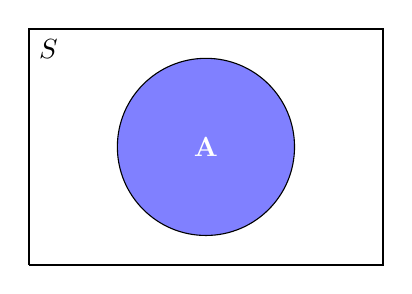
\begin{tikzpicture}[scale=1.5]
			 \draw[thick] (0,0)--(0,2)node[below right]{$S$}--(3,2)--(3,0)--(0,0);
			 \draw[black, fill=blue!50] (1.5,1) circle (0.75cm)node{\textcolor{white}{$\textbf{A}$}};
		\end{tikzpicture}	
		\caption*{The sample space $S$ and event $A$. $P(S)=1$}
	\end{figure}
	\item Probability Rules
	\begin{enumerate}
			\item $0 \leq P \leq 1$
			\item $P(S)=1$
			\item The probability of an event $\textbf{A}$ \emph{not} occurring, $P(\neg \textbf{A}) =1-P(\textbf{A})$ is the complement of \textbf{A}
			\begin{itemize}
				\item e.g. if the probability of picking a blue M\&M is 	$P(Blue)=0.47$, the probability of picking a \emph{not} blue M\&M is $P(\neg Blue)=0.53$
			\end{itemize}
\clearpage
	\begin{figure}[h!]
		\centering
		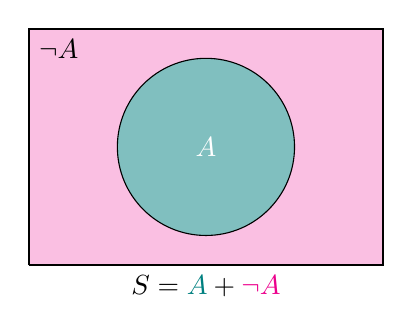
\begin{tikzpicture}[scale=1.5]
			\draw[fill=magenta!25](0,0)--(0,2)--(3,2)--(3,0)--(0,0);
			\draw[thick] (0,0)--(0,2)--(3,2)--(3,0)--(0,0);
			 \draw[thick] (0,0)--(0,2)node[below right]{$\neg A$}--(3,2)--(3,0)--node[below]{$S=\textcolor{teal}{A}+\textcolor{magenta}{\neg A}$}(0,0);
			 \draw[black, fill=teal!50] (1.5,1) circle (0.75cm)node{\textcolor{white}{$A$}};
		\end{tikzpicture}	
		\caption*{The event \textbf{A} in teal and its complement $\neg\textbf{A}$ in red}
	\end{figure}
			\item \textbf{Generalized Addition Rule}:
			\begin{equation*}P(\textbf{A} \text{ or } \textbf{B}) = P(\textbf{A}) + P(\textbf{B}) - P(\textbf{A} \text{ and } \textbf{B})\end{equation*}
				\begin{figure}[h!]
		\centering
		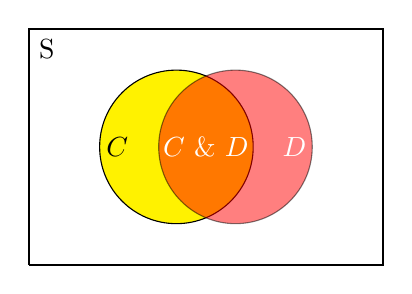
\begin{tikzpicture}[scale=1.5]
			 \draw[thick] (0,0)--(0,2)node[below right]{S}--(3,2)--(3,0)--(0,0);
			 \draw[black, fill=yellow] (1.25,1) circle (0.65cm);
			 \draw[black, fill=red, opacity=.5] (1.75,1) circle (0.65cm);
			 \draw[white] (1.5, 1)node{$C$ \& $D$};
			 \draw[black] (.75, 1)node{$C$};
			 \draw[white] (2.25,1)node{$D$};
		\end{tikzpicture}	
		\caption*{Non-disjoint events, e.g. The probability of picking a face card (\textbf{C}) OR a heart card (\textbf{D}) is: the probability of a heart plus the probability of a face minus the probability of cards that are both}
	\end{figure}
			\begin{itemize}
				\item The symbol for ``OR'' is $\cup$, the union of two disjoint events. The symbol for ``AND'' is $\cap$, the intersection (overlap) of two events. So the generalized addition rule is:
			\begin{equation*}P(\textbf{A} \cup \textbf{B}) = P(\textbf{A}) + P(\textbf{B}) - P(\textbf{A}\cap \textbf{B})\end{equation*}
				\item If $P(\textbf{A} \text{ and } \textbf{B})=0$, then \textbf{A} and \textbf{B} are \textbf{disjoint} 
				\begin{itemize}
					\item Disjoint events cannot occur simultaneously, e.g. picking one M\&M that is BOTH red AND blue
				\end{itemize}
				\item If two events are disjoint--the \textbf{\emph{simple} addition rule} (because $P(\textbf{A} \text{ and } \textbf{B})=0$):
							\begin{equation*}P(\textbf{A} \text{ or } \textbf{B}) = P(\textbf{A}) + P(\textbf{B}) \end{equation*}
			\end{itemize}
			\begin{figure}[h!]
				\centering 
			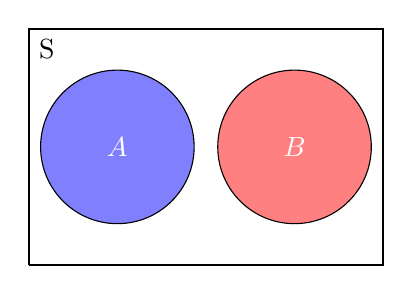
\begin{tikzpicture}[scale=1.5]
			 \draw[thick] (0,0)--(0,2)node[below right]{S}--(3,2)--(3,0)--(0,0);
			 \draw[black, fill=blue!50] (0.75,1) circle (0.65cm)node{\textcolor{white}{$A$}};
			 \draw[black, fill=red!50] (2.25,1) circle (0.65cm)node{\textcolor{white}{$B$}};
		\end{tikzpicture}	
		\caption*{Disjoint events $\textbf{A}$ and $\textbf{B}$}
			\end{figure}
			\clearpage
	\item \textbf{Conditional Probability:} 
			\begin{equation*}
		P(\textbf{B}|\textbf{A})=\frac{P(\textbf{A} \text{ and } \textbf{B})}{P(\textbf{A})}
		\end{equation*}
		\begin{itemize}
			\item ``The probability of event \textbf{B} \emph{given} ($|$) event \textbf{A}''
			\item e.g. the probability of someone watching the Super Bowl, \emph{given} that they are male 
		\end{itemize}
\item \textbf{Generalized Multiplication Rule}: 
		\begin{equation*}P(\textbf{C} \text{ and } \textbf{D}) = P(\textbf{C})*P(\textbf{D}|C)\end{equation*}
			\begin{itemize}
				\item If $P(\textbf{D}| \textbf{C})=P(\textbf{D})$, then \textbf{C} and \textbf{D} are \textbf{independent} (\textbf{C}'s occurrence does not change P(\textbf{D}))
				\begin{itemize}
					\item Independent events: if one event occurring gives \emph{no} information about the probability of another event
				\end{itemize}
				\item If \textbf{C} and \textbf{D} are independent, the \textbf{\emph{Simple} Multiplication Rule}:
							\begin{equation*}P(\textbf{C} \text{ and } \textbf{D}) = P(\textbf{C}) * P(\textbf{D}) \end{equation*}
				\item Independent $\neq$ Disjoint! Disjoint events \emph{cannot} be independent!
				\begin{itemize}
					\item If events  \textbf{A} and \textbf{B} are disjoint ($P(\textbf{A} \cap \textbf{B})=0)$, this implies that if \textbf{A} occurs, \textbf{B} cannot possibly occur (mutually exclusive!) so $P(\textbf{B}|\textbf{A})=0\neq P(\textbf{B})$
					\item e.g. If you get an A in this course, that means the probability of you getting a B, C, D, or F$=0$! 
				\end{itemize}
			\end{itemize}
\end{enumerate}
\end{itemize}

\section{Contingency Tables, Joint \& Marginal Probability} 
\begin{itemize}
	\item Contingency tables display the joint and marginal distributions of two variables 
			\begin{table}[h!]
			\centering 
			\begin{tabular}{lrrr}
			& \multicolumn{2}{c}{\# of Bedrooms} & \\ \cmidrule{2-3}
			Price & 1 & 2 & \textbf{Total}\\ \toprule 
			Low & 0.30 & 0.20 & \textbf{0.50}\\
			High & 0.10 & 0.40 & \textbf{0.50}\\ \midrule 
			\textbf{Total} & \textbf{0.40} & \textbf{0.60} & \textbf{1.00} \\ \bottomrule 
			\end{tabular}
		\end{table}
	\begin{itemize}
		\item Each cell is a disjoint union of events with a \textbf{joint probability} 
		\begin{itemize}
			\item e.g. $P(\text{Low Price} \cap \text{1 Bedroom})=0.30$, given by the table 	
		\end{itemize}
		\item \textbf{Marginal probabilities} are the probability of each category occurring overall, in margin of table
		\begin{itemize}
			\item e.g. P(1 Bedroom)=0.40; P(Low)=0.50
		\end{itemize} 
		\item \textbf{Conditional distribution} (e.g. of price) can be calculated with conditional probabilities for one condition (e.g. for an apartment having 2 Bedrooms)
		\begin{equation*}
		P(\text{Low Price}|\text{2 Bedrooms})=\frac{P(\text{Low Price}\cup \text{2 Bedrooms})}{P(\text{2 Bedrooms)}}=\frac{0.20}{0.60}=0.33	
		\end{equation*}
		\begin{equation*}
		P(\text{High Price}|\text{2 Bedrooms})=\frac{P(\text{High Price}\cup \text{2 Bedrooms})}{P(\text{2 Bedrooms)}}=\frac{0.40}{0.60}=0.67	
		\end{equation*}
\end{itemize}
\end{itemize}

\clearpage 

\section{Bayes' Rule} 
\begin{itemize}
	\item We know $P(B|A)$ but may want to find $P(A|B)$, they are not the same! 
	\item \textbf{Bayes' Rule}: 
			\begin{equation*}
		P(A|B)=\frac{P(B|A)P(A)}{P(B)}	
		\end{equation*}
		\item We often don't know $P(B)$ (the denominator). We use the \textbf{law of total probability}, if we know $B$ can occur simultaneously with either $A$ or $\neg A$:
				\begin{equation*}
		P(B)=P(B|A)P(A)+P(B|\neg A)P(\neg A)	
		\end{equation*}
		\begin{figure}[h!]
		\centering 
		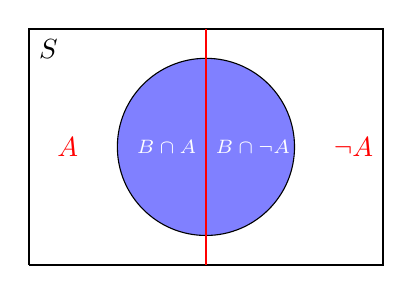
\begin{tikzpicture}[scale=1.5]
			 \draw[thick] (0,0)--(0,2)node[below right]{$S$}--(3,2)--(3,0)--(0,0);
			 \draw[black, fill=blue!50] (1.5,1) circle (0.75cm);
			  \draw[white] (1.5,1)node[left]{\scriptsize $B \cap A$};
			  \draw[white] (1.5,1)node[right]{\scriptsize $B \cap \neg A$};
			 \draw[red](1.5,0)--node[left=1.5cm]{$A$}node[right=1.5cm]{$\neg A$}(1.5,2);
		\end{tikzpicture}	
	\end{figure}
	\item Example: Suppose 1\% of the population has a rare disease. A test that can diagnose the disease is 95\% accurate. What is the probability that a person who takes the test and comes back positive has the disease? [Stop and try to think through this before proceeding. Your intuitions will fail you!] 
		\begin{equation*}
		P(Disease|Positive)=\frac{P(Positive|Disease)P(Disease)}{P(Positive)}	
		\end{equation*}	
	\begin{itemize}
		\item We know $P(Positive|Disease)=0.95$, $P(Disease)=0.01$, what is $P(Positive$)? 
		\item Find using law of total probability: 
		\begin{equation*}
		P(Positive)=P(Positive|Disease)P(Disease)+P(Positive|No Disease)P(No Disease)
		\end{equation*}
		\begin{equation*}
		P(Positive)=0.95*0.01+0.05*0.99=0.0095+0.0495=0.0590	
		\end{equation*}
		\item So finally: 
		\begin{equation*}
		P(Disease|Positive)=\frac{0.95*0.01}{0.059}=0.16	\implies 16\%! 
		\end{equation*}
		\item The magic of Bayes' rule is that everyone forgets the base rate (the disease itself is so rare). 
	\end{itemize}
	\item In Bayesian updating: 
	\begin{itemize}
          \item $P(A)$ is the ``base rate'' or ``prior''
          \item $P(A|B)$ is the ``posterior,'' having accounted for $\textbf{B}$
          \item $P(B|A)$ is the ``likelihood'' of A and B being compatible
          \item $P(A)$ is the ``marginal likelihood'' of (all possible events of) A irrespective of B
     \end{itemize}
     \item Most important to remember $P(A|B) \neq P(B|A)$! 
\end{itemize}


\end{document}
